\documentclass[a4paper, 11pt]{article}
\usepackage{graphicx} % Required for inserting images
\usepackage[portuguese]{babel}

\title{BD-PL02}
\author{Eduardo Fernandes}
\date{2025}

\begin{document}

\maketitle

\noindent \textbf{Exercício 1}\\

\noindent Joana Prior necessita de um sistema de base de dados para gerir os artigos sobre o ator, pois, após o acumular de artigos, as consultas a estes tornaram-se ineficientes, e ao estabelecer um método de organização da informação, aceder à informação desejada deixará de ser um problema. É também importante realçar a capacidade de escalar a base de dados para maiores capacidades, sem prejudicar a sua eficiência.\\

\noindent \textbf{Exercício 2}\\

\noindent Lista de requisitos de Descrição:

\begin{itemize}
    \item Um \textbf{artigo} deve ser registado com a sua identificação (um código estruturado de acordo com a natureza do próprio artigo), o seu título, um pequeno resumo da notícia, as fotografias incluídas no texto, se existentes, a rede social na qual foi publicado e a data da sua publicação;
    \item Cada \textbf{filme} é caracterizado por um identificador único, nome, data de lançamento e realizador;
    \item Cada \textbf{categoria} de artigo é caracterizada por um identificador único e a sua designação;
    \item Um \textbf{autor} é descrito por um identificador único, nome e data de nascimento;
\end{itemize}

\newpage

\noindent \textbf{Exercício 3}\\

\noindent Através dos requisitos de Descrição apresentados acima, podemos desenhar o seguinte esquema conceptual:

\begin{figure}[h]
    \centering
    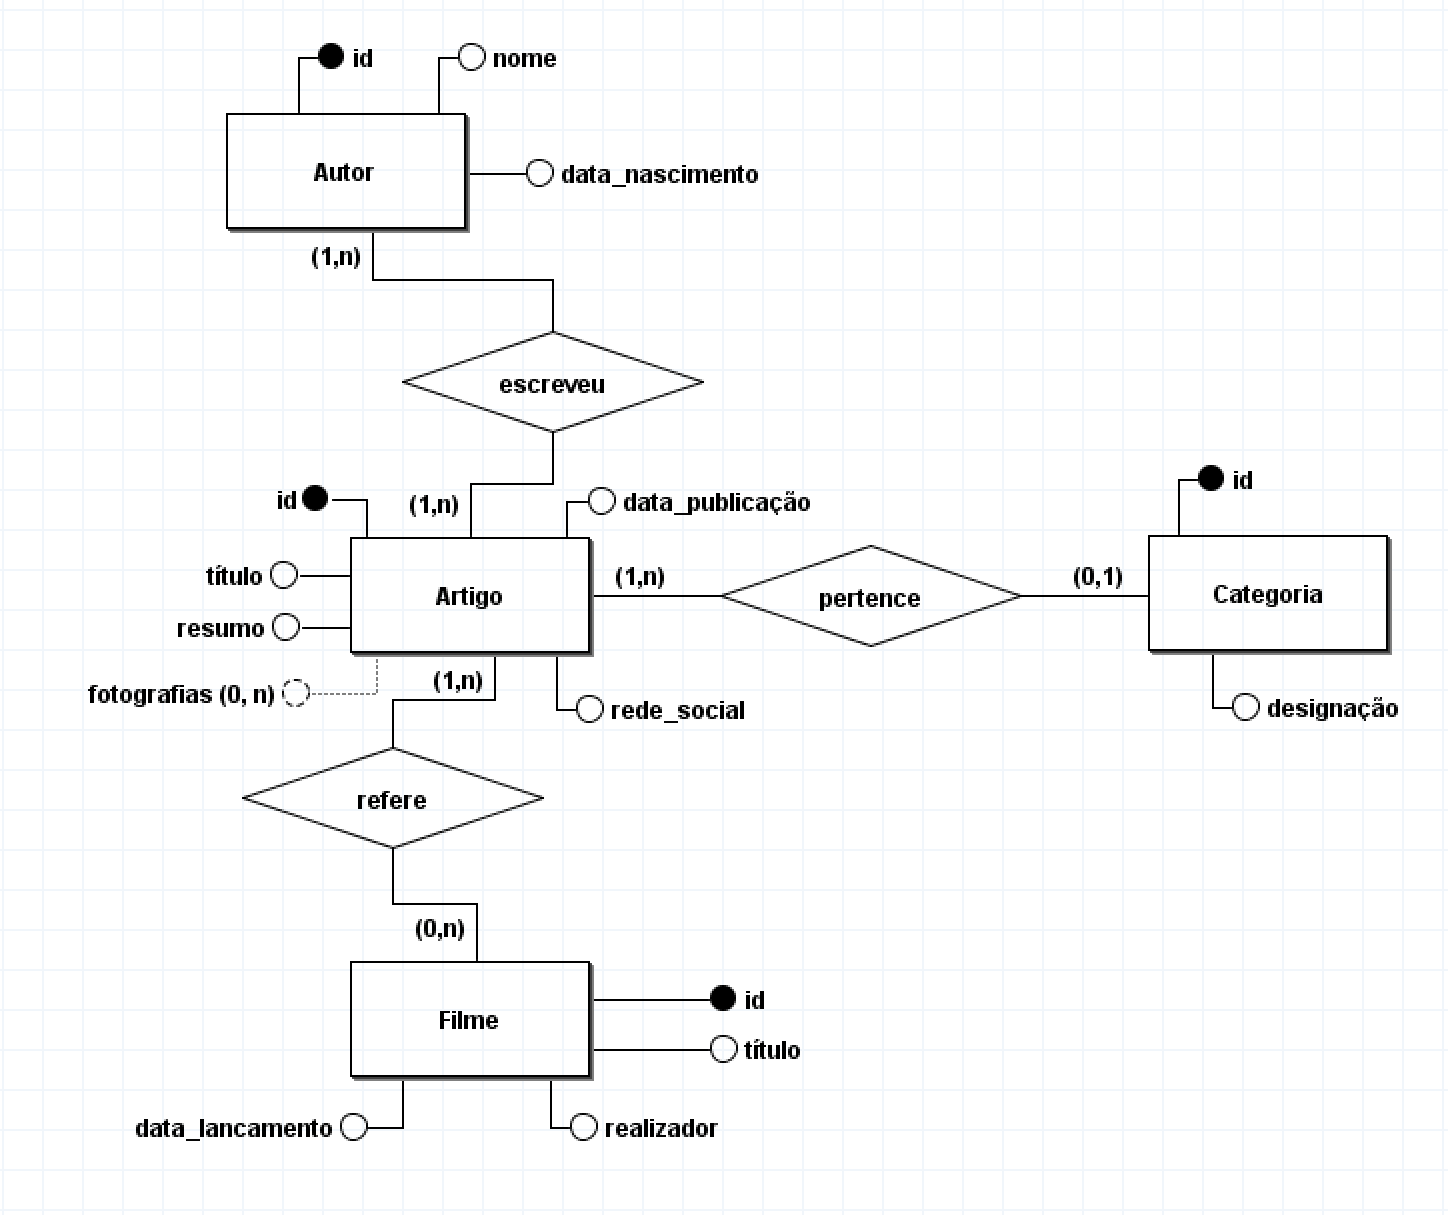
\includegraphics[width=1\linewidth]{modelo-pl02.png}
    \caption{Modelo Conceptual}
\end{figure}

\end{document}
